\documentclass{izpit}

\begin{document}

%==========================================================================
%               Sem vpisi podatke o izpitu
%==========================================================================
\FRACTIONSIMPLIFY{31}{1}{\skupnotock}{\nepomembno}%Sem vpiši (v polje trenutno {60}) skupno število točk, da paket naračuna kriterij ocenjevanj
\izpit[ucilnica = RAZRED, naloge = 6]%ucilnica RAZRED, lahko se sedezni red, ime in priimek, maturitetni
{Matematika - Zaporedja}{22. 9. 2023}{Čas pisanja je 45 minut.\\ Možno je doseči $\skupnotock$ točk.\\ Veliko uspeha!}
%==========================================================================
%               Nepomembno - Preskoči
%==========================================================================
\MAX{0.1}{0}{\tempepsilon}%shranimo epsilon... ne gre trik z ulomkom zato max
\MULTIPLY{\skupnotock}{0.9}{\odlicno}
\MULTIPLY{\skupnotock}{0.76}{\pravdobro}
\MULTIPLY{\skupnotock}{0.63}{\dobro}
\MULTIPLY{\skupnotock}{0.5}{\zadostno}
\ADD{\dobro}{\tempepsilon}{\dobroplus}
\ADD{\pravdobro}{\tempepsilon}{\pravdobroplus}
\ADD{\odlicno}{\tempepsilon}{\odlicnoplus}
\ROUND[0]{\dobroplus}{\dobroplus}
\ROUND[0]{\pravdobroplus}{\pravdobroplus}
\ROUND[0]{\odlicnoplus}{\odlicnoplus}
\ROUND[0]{\zadostno}{\zadostno}
\ROUND[0]{\dobro}{\dobro}
\ROUND[0]{\pravdobro}{\pravdobro}
\ROUND[0]{\odlicno}{\odlicno}\begin{small}
 \PlaceText{100mm}{33mm}{\begin{tabular}{ll}
    \multicolumn{2}{c}{\textbf{Kriterij ocenjevanja}} \\[0.5ex]
    Ocena & Tocke \\ \hline
    zadostno & $\zadostno - \dobro$ \\
    dobro & $\dobroplus - \pravdobro$ \\
    prav dobro & $\pravdobroplus - \odlicno$ \\
    odlicno & $\odlicnoplus$--
  \end{tabular}}\end{small}
 \ifthenelse{\boolean{@maturitetni}}{\newpage}%TO JE ZELO GRDA KODA a ker ne gre kriterij v class ni druge moznosti
%==========================================================================
%               Sem vpisi naloge
%   za dodatek koordinatnega sistema daj pod navodila naloge \dodatek{\[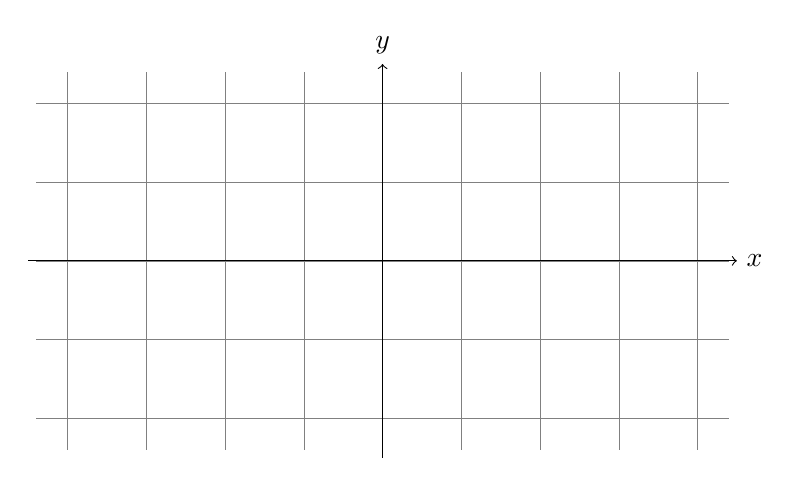
\begin{tikzpicture}
        \draw[help lines,step=1cm] (-4.4,-2.4) grid (4.4,2.4);
        \draw[->] (-4.5,0) -- (4.5,0) node[right] {$x$};
        \draw[->] (0,-2.5) -- (0,2.5) node[above] {$y$};
\end{tikzpicture}\]}
%   oz. za kompleksno ravnino \dodatek\[\begin{tikzpicture}
        \draw[help lines,step=1cm] (-4.4,-2.4) grid (4.4,2.4);
        \draw[->] (-4.5,0) -- (4.5,0) node[right] {$Re$};
        \draw[->] (0,-2.5) -- (0,2.5) node[above] {$Im$};
\end{tikzpicture}\]
%==========================================================================

\naloga[\tocke{8}]
  \podnaloga[4]
  Zaporedju, danemu s splošnim členom $a_n=\frac{4n}{n+1}$, določi natančno zgornjo in spodnjo mejo in ju dokaži.
  \prostor[1]
  \podnaloga[4]
  Poišči limito zaporedja in izračunaj, koliko členov leži izven $\varepsilon$-okolice limite, če je $\varepsilon=\frac{7}{100}$.
  \prostor[1]
  \naloga*[\tocke{3}]
  Pokaži, da je zaporedje $b_n=2^n-1$ naraščajoče.
  \prostor[1]

  
\naloga[\tocke{2}]
  Za aritmetično zaporedje $a_n=2n-2$ izračunaj vsoto $\sum_{n=1}^{100} a_n =a_1 +\ldots +a_{100}$.
  \prostor[1]
  \naloga*[\tocke{5}]
  Določi $x\in\mathbb{R}$, da bodo $3x+2$, $x-6$ in $3x-4$ zaporedni členi geometrijskega zaporedja. Zapiši zaporedji in določi količnik $k$.
  \prostor[3]


\naloga[\tocke{5}]
  Z matematično indukcijo pokaži, da $3$ deli $2^{2n}-1$ za vsak $n\in \mathbb{N}$.
  %\prostor[2]
  %\podnaloga[dodatne 3 točke]
  %Pokaži, da lahko vsako $2^n\times 2^n,\ n\in\mathbb{N}$ ploščo pokrijemo s ploščami oblike L, ki zasedejo 3 ploščice, kjer en kvadratek (na poljubnem mestu) lahko izpustimo. Primer za $4\times 4$ prikazuje slika.
  %\begin{figure}[H]
  %\centering
  %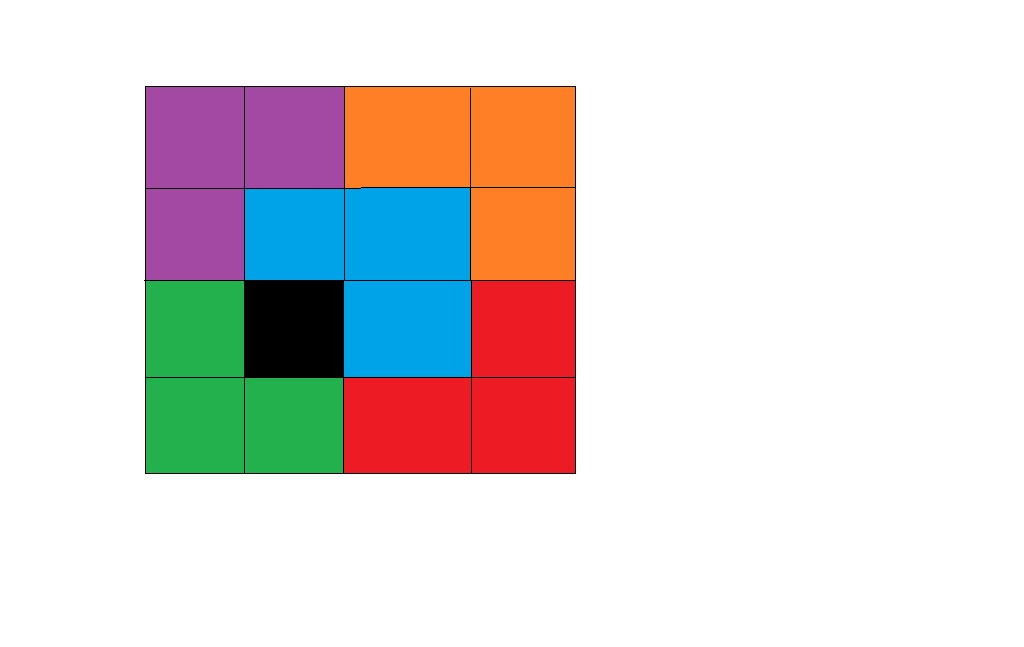
\includegraphics[width =0.3\textwidth]{naloga.jpg}
  %\end{figure}
  %\prostor[1]


\naloga[\tocke{8}]
  \podnaloga[4]
  Za koliko časa moramo na banko vložiti $10000\euro{}$, da na koncu dobimo $3000\euro{}$ obresti, če je kapitalizacija mesečna. Letna obrestna mera je $6\%$.
  \prostor[1]
  \podnaloga[4]
  Danes vzamemo kredit v višini $12000\euro{}$, ki ga bomo odplačevali mesečno dve leti. Prvi obrok bomo plačali čez en mesec. Izračunaj mesečni obrok (anuiteto), če je letna obrestna mera je $6\%$.
  \prostor[1]



\end{document}